\section{Core1990}
\label{Appendix:Core1990}
Core1990 is a point-to-point communication protocol using the royalty-free Interlaken protocol as it's foundation. It is designed by engineers and students of the Electronics Department of Nikhef (Amsterdam, The Netherlands) with large experiments at CERN (e.g. ATLAS) in mind. \\
The development of Core1990 was intended to publish an open source protocol providing high throughput with a small percentage of overhead. Certain features like flow control and error detection are included.\\

This document will describe setting up the core including configurations of IP-cores included in the design. During development and writing this document a Xilinx VC707 evaluation board is used and sometimes certain IO's will be referred to. This is of course board dependent and these are mentioned as examples to clear things up.

\begin{figure}[H]
	\centering
	
\includegraphics[width=.7\textwidth]{Core1990/Core1990_logo.jpg}	
	\caption{Core1990 logo}
	\label{fig:Core1990_logo}
\end{figure} 

\subsection{Features}
	Core1990 is packed with a lot of features providing among others data integrity and detection of errors while transmitting. These features are designed to be compliant with those featured in the Interlaken protocol definition. 
	
	\begin{itemize}
		\item Lane rate transceiver dependent
		\item Support framing consistent with the Interlaken Protocol Definition
		\item Generates CRC-24 and CRC-32 for error checking
		\item 58-bit independent synchronous scrambler
		\item 64b/67b encoding
		\item About 90\% bandwidth efficiency possible (depends on user configuration)
		\item Self-synchronizing links
		\item Flow control
	\end{itemize}
	
\newpage
	
\subsection{Obtaining and building Core 1990}
	Implementing the core in a design can be done easily by using the files provided with core1990.
	The complete process of obtaining and building Core1990 will be described including which files are required and should be included. The project has been designed in Xilinx Vivado 16.4 but should be compatible with other versions. The correct configuration of the ip cores will also be mentioned to ensure behavior as expected.
	
	The complete project can be downloaded through the download link on the OpenCores site itself or through SVN. For OpenCores the link is \href{https://opencores.org/project/core1990_interlaken}{https://opencores.org/project/core1990\\\_interlaken} and the SVN links is \href{https://opencores.org/ocsvn/core1990_interlaken/core1990_interlaken/trunk}{https://opencores.org/ocsvn/core1990\_interlaken/core1990\\\_interlaken/trunk} in case this is preferred.\\
	
	 \begin{forest}
	 	pic dir tree,
	 	where level=0{}{% folder icons by default; override using file for file icons
	 		directory,
	 	},
	 	[Core1990
		 	[constraints]
		 	[scripts]
		 	[simulation]
		 	[sources
			 	[Interlaken\_Interface.vhd, file]
			 	[ip\_cores
				 	[clk\_40MHz.xci, file]
				 	[RX\_FIFO.xci, file]
				 	[Transceiver\_10g\_64b67b.xci, file]
				 	[TX\_FIFO.xci, file] ]
			 	[CRC
				 	[crc-24.vhd,file]
				 	[crc-32.vhd, file] ]
			 	[Receiver
				 	[interlaken\_receiver.vhd,file]
				 	[decoder.vhd, file]
				 	[deframing\_burst.vhd, file]
				 	[deframing\_meta.vhd, file]
				 	[descrambler.vhd, file] ] 
			 	[Transmitter
			 		[interlaken\_transmitter.vhd,file]
			 		[encoder.vhd, file]
			 		[framing\_burst.vhd, file]
			 		[framing\_meta.vhd, file]
			 		[scrambler.vhd, file] ]
	 		] 
	 	]
	 \end{forest}
	
	The directory tree depicts the file structure in the sources folder. This should contain several files to configure the ip cores, a folder containing two crc error detection modules, a receiver and transmitter folder containing the module files. A main file is included in the folder that is meant for the top level connecting all modules correctly to each other.
	
	Besides these files there are also three different folders. One contains the constraints which are responsible for connecting the physical pins to the signals in the package and providing clock information to the fitter of the design. Another folder contains several scripts to build the project by just running a single script. Another script will be able to generate testbenches on request of the user and a script generates the implementation of the design. The simulation folder contains a lot of testbenches used to simulate all the components included in the design.\\
	
	\begin{forest}
		pic dir tree,
		where level=0{}{% folder icons by default; override using file for file icons
			directory,
		},
		[Core1990
			[constraints
				[Core1990\_Constraints.xdc, file] ]
			[scripts
				[implementation.tcl, file]
				[simulation.tcl, file]
				[vivado\_import\_virtex7.tcl, file]	]
			[simulation]
			[sources] 	
		]
	\end{forest}

	\vspace{1mm}
	For building the project Vivado has to be opened and the vivado\_import\_virtex7.tcl has to be executed. This can be done by changing the directory in the tcl console to the scripts folder and then giving the command 'source vivado\_import\_virtex7.tcl'. This will add the project folder to the directory tree and contains the just generated project. 
	
	When the project has been imported in vivado the structure should match the one depicted in Figure \ref{fig:Core1990_VivadoCore}.
	
	\begin{figure}[H]
		\centering
		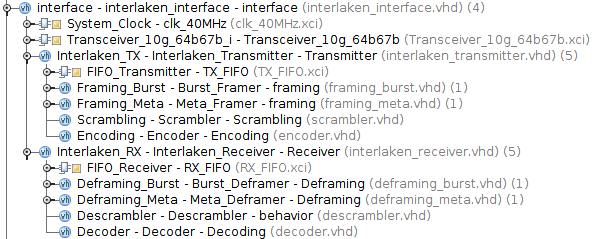
\includegraphics[width=\textwidth]{Core1990/Core1990_VivadoCore.png}
		\caption{Structure of the project in Vivado}
		\label{fig:Core1990_VivadoCore}
	\end{figure}

\newpage
\subsection{Transceiver IP Core}
	Configuring the transceiver is an essential step in setting up the core. This will describe the correct settings to use for the functional behavior of the protocol. In case the transceiver is configured in a wrong way, no data or corrupted data will arrive at the receiving side. This section will guide the user to set up the transceiver in an easy way without adjusting too many clocks, targeting the VC707 board.\\
	
	The transceiver core can be configured by browsing through a separate window that will pop up. The fist tab named GT Selection should already have the GTX as GT Type selected and the shared logic should be included in the core, not the example design.
	
	After this the second tab will provide more important options. The line rate should be set to 10 Gbps while the reference clock can be set at 125 MHz. This clock is available on the board at IO pins AH7 and AH8, REFCLK0\_Q0. Using the QPLL GTX X1Y2 can be used. Figure \ref{fig:IP_TransceiverConf1} shows the correct configuration.
	
	\begin{figure}[H]
		\centering
		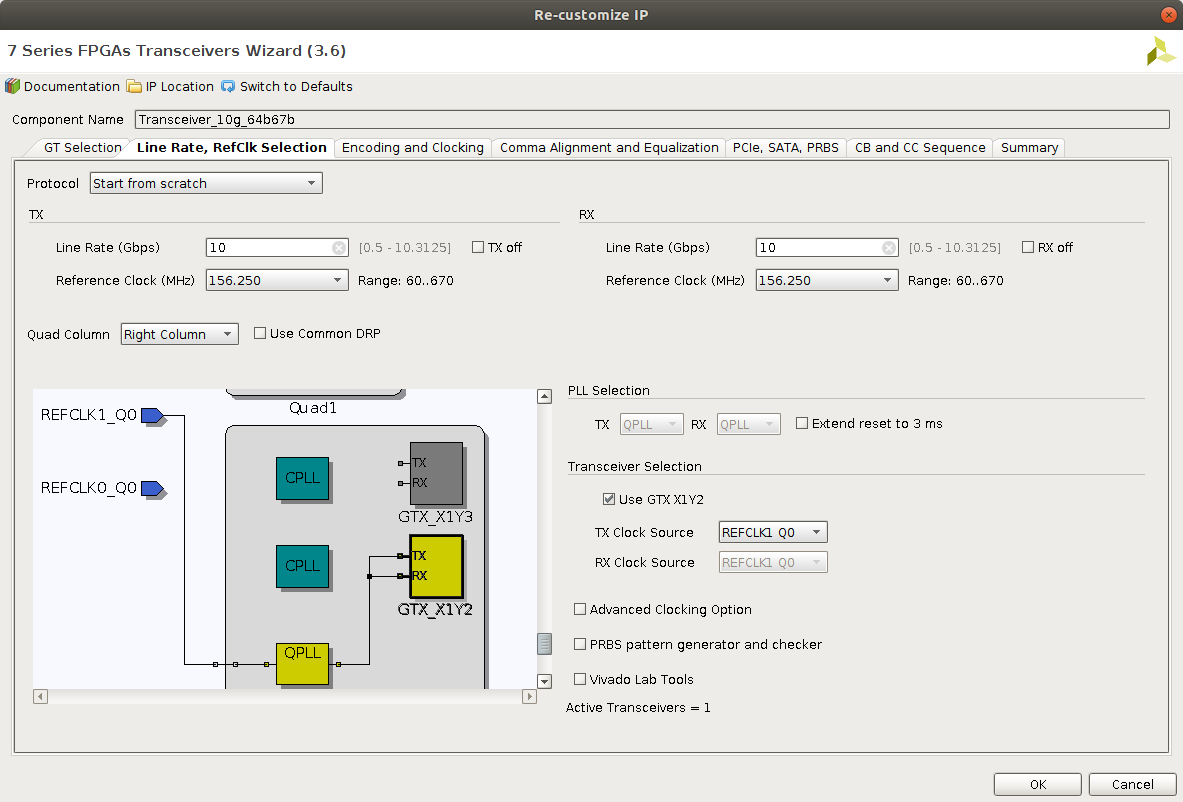
\includegraphics[width=\textwidth]{Core1990/IP_TransceiverConf1.png}	
		\caption{Transceiver lane rate and reference clock selection}
		\label{fig:IP_TransceiverConf1}
	\end{figure} 
	
	The encoding and clocking tab shows other important settings. For both the TX and RX, the external data width should be set at 64-bits while the internal data width is 32 bits. Encoding has to be set at 64B/67B with Internal Sequence Counter and decoding has to be set at 64B/67B. The DRP/System Clock Frequency has to be set at 40 MHz. Figure \ref{fig:IP_TransceiverConf2} shows the right settings.
	
	\begin{figure}[H]
		\centering
		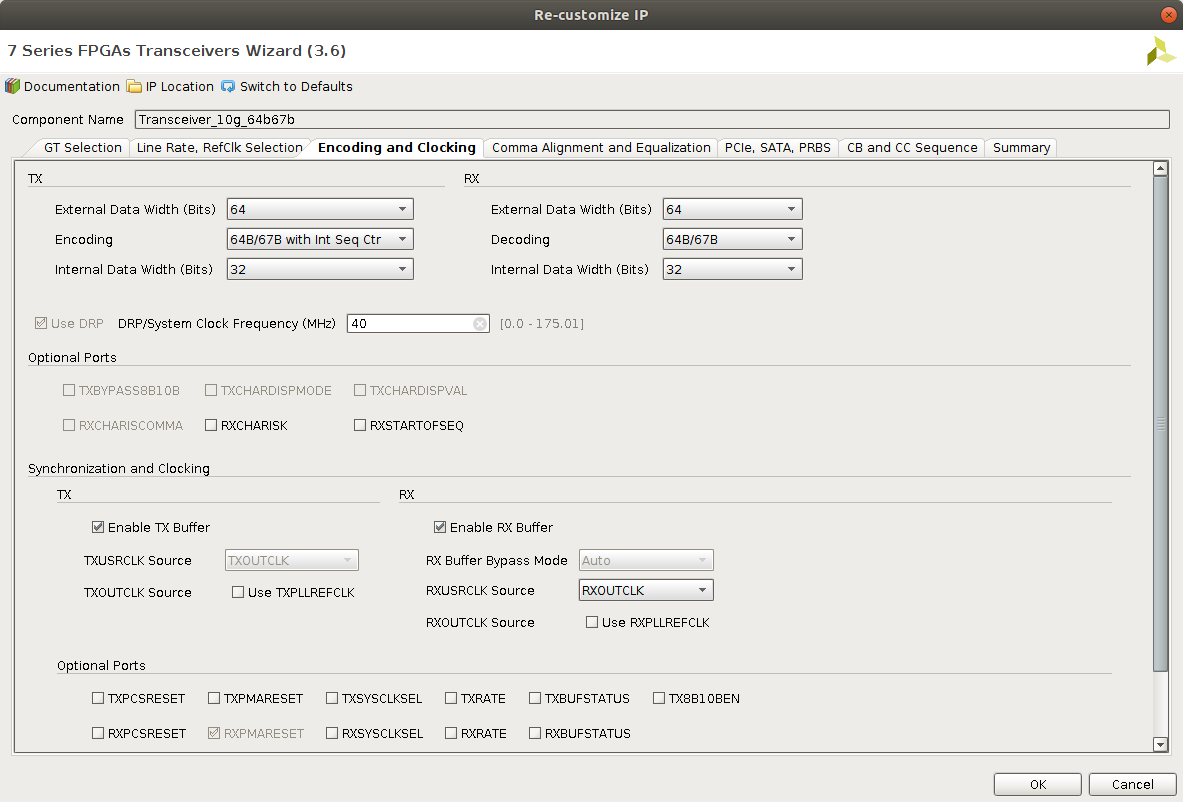
\includegraphics[width=0.95\textwidth]{Core1990/IP_TransceiverConf2.png}	
		\caption{Transceiver encoding and system clock selection}
		\label{fig:IP_TransceiverConf2}
	\end{figure} 
	
	The other tabs are not important and no settings should be changed in these tabs. Figure \ref{fig:IP_TransceiverConf3} shows a complete summary of the features included with the transceiver when this core will be generate. The user should have the same settings on screen. 
	
	\begin{figure}[H]
		\centering
		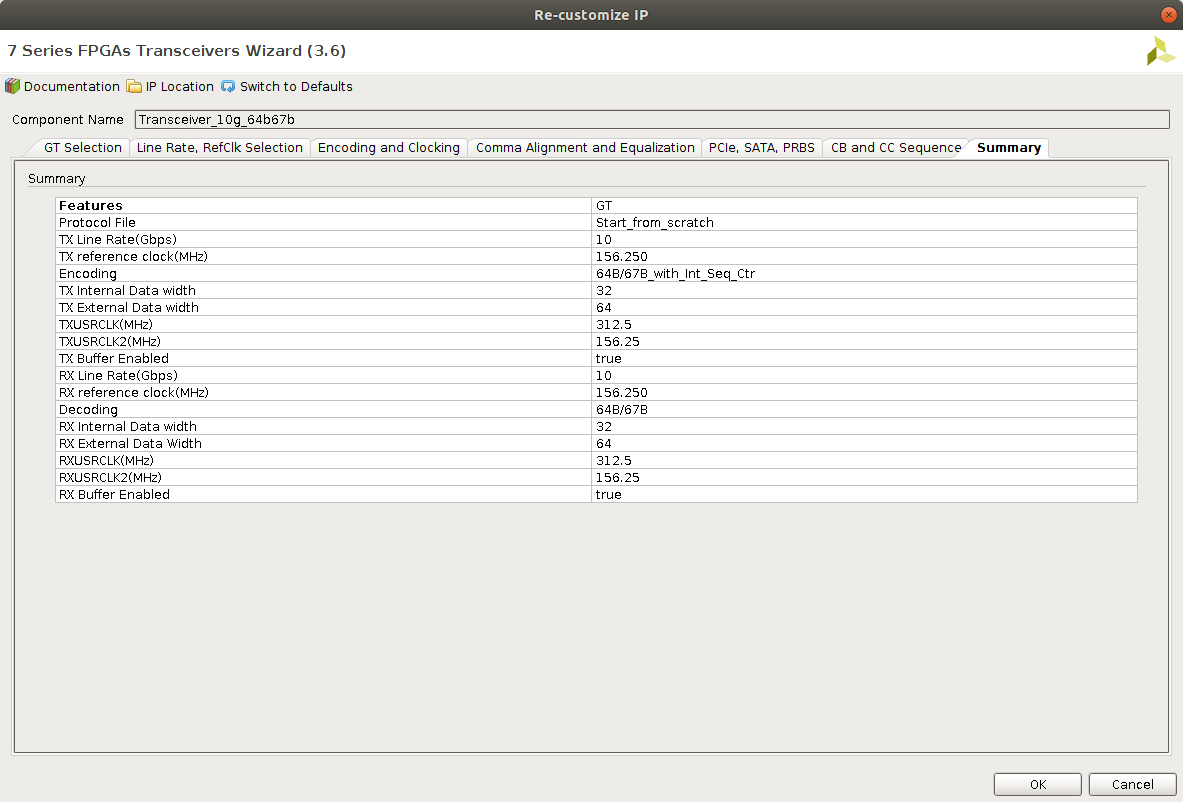
\includegraphics[width=0.95\textwidth]{Core1990/IP_TransceiverConf3.png}	
		\caption{Transceiver summary of configuration}
		\label{fig:IP_TransceiverConf3}
	\end{figure} 

\newpage

\subsection{Clocking Wizard IP Core}
	The system clock will be generated using a clock input provided to the chip. In this case this is a 200 MHz input at IO pins E18 and E19. The frequency will be scaled down using the Xilinx Clocking Wizard which generates an IP core. Two clocks will be provided in this case. One will end up being the DRP clock of the transceiver and another clock will be the clock selected by the user. This clock can be connected to external user logic, for example a data generator, or the FIFO write and FIFO read on respectively the TX and RX side.
	 
	\begin{figure}[H]
		\centering
		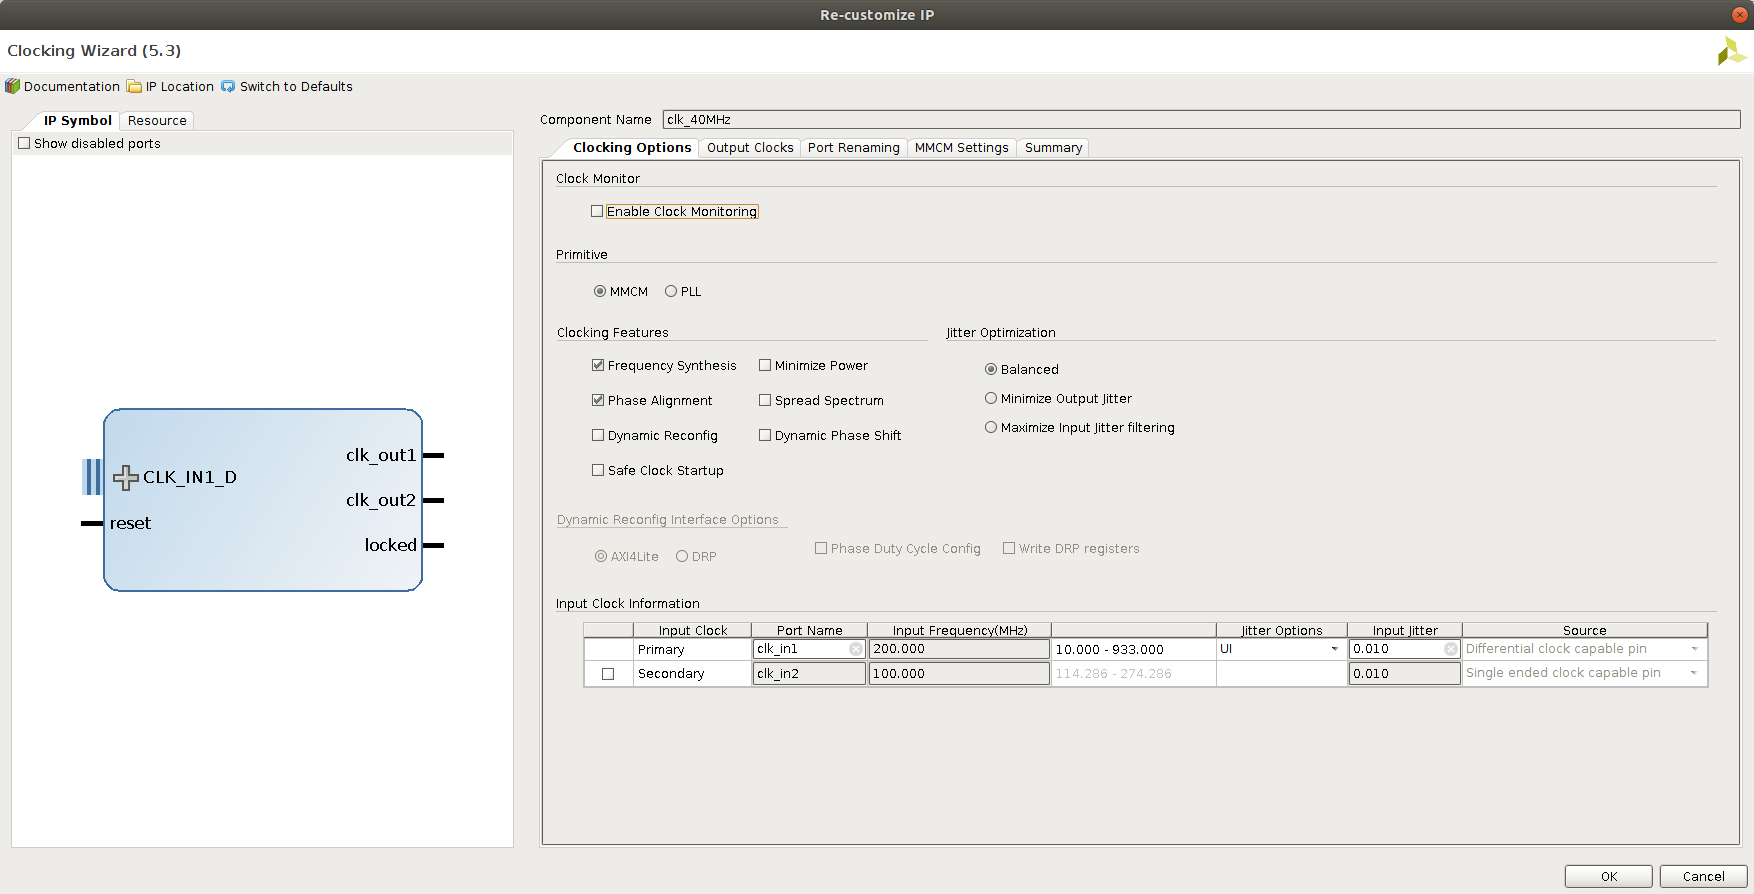
\includegraphics[width=\textwidth]{Core1990/IP_CLK40Conf1.png}
		\caption{Clocking wizard input clock(s) and features}
		\label{fig:IP_CLK40Conf1}
	\end{figure}
	
	The first tab of the clocking wizard provides some basic information on the input clock which in this case will be a 200 MHz differential clock. It is important to select 'differential clock capable pin' under source here. This core makes use of a MMCM (Mixed-Mode Clock Manager). From clocking features only Frequency synthesis and phase alignment are selected. The jitter optimization is balanced and the input frequency of the primary clock is 200MHz. There is no secondary clock to use thus this is not selected and relevant. Figure \ref{fig:IP_CLK40Conf1} shows the configuration on the first tab. \\

	The second tab will provide more configuration on the output clocks. Like depicted in Figure \ref{fig:IP_CLK40Conf2} there will be one 40 MHz clock and this has to stay at 40 MHz. Another clock is set at 150 MHz but this is the clock available for user logic like mentioned earlier. This can be configured as reference frequency to send data packets at. It is up to the user to determine whether this clock will be used and at which frequency it will run. However the maximum frequency of this clock also determines on the lane rate of the transceiver and at which speed the Interlaken interface itself runs. The example design in \ref{Appendix:Core1990_ExampleDesign} will also use this clock and describe more on it's usage. All clocks use a duty cycle of 50\% and from the optional outputs only the reset and locked pins are required.
	
	\begin{figure}[H]
		\centering
		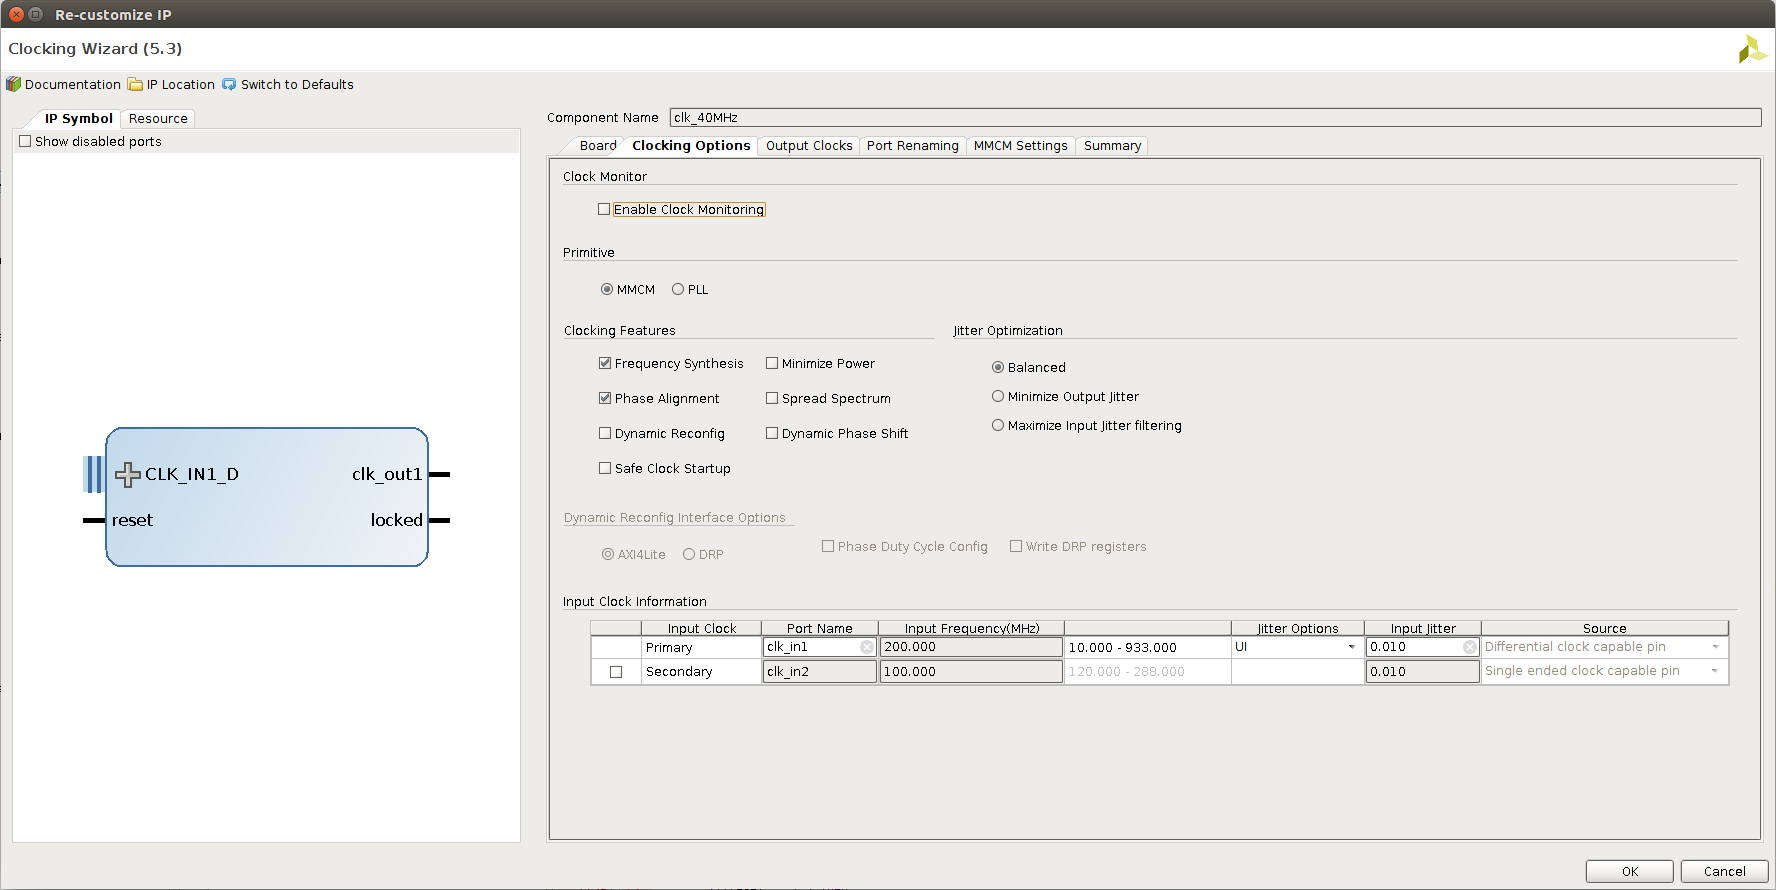
\includegraphics[width=\textwidth]{Core1990/IP_CLK40Conf2.png}	
		\caption{Clocking wizard output clocks}
		\label{fig:IP_CLK40Conf2}
	\end{figure} 
	
	The last important tab is the summary tab. This should give an overview that contains the same information and values as depicted in Figure \ref{fig:IP_CLK40Conf3}. However if the second output clock is set at another frequency this will of course give a different value is the overview.
		
	\begin{figure}[H]
		\centering
		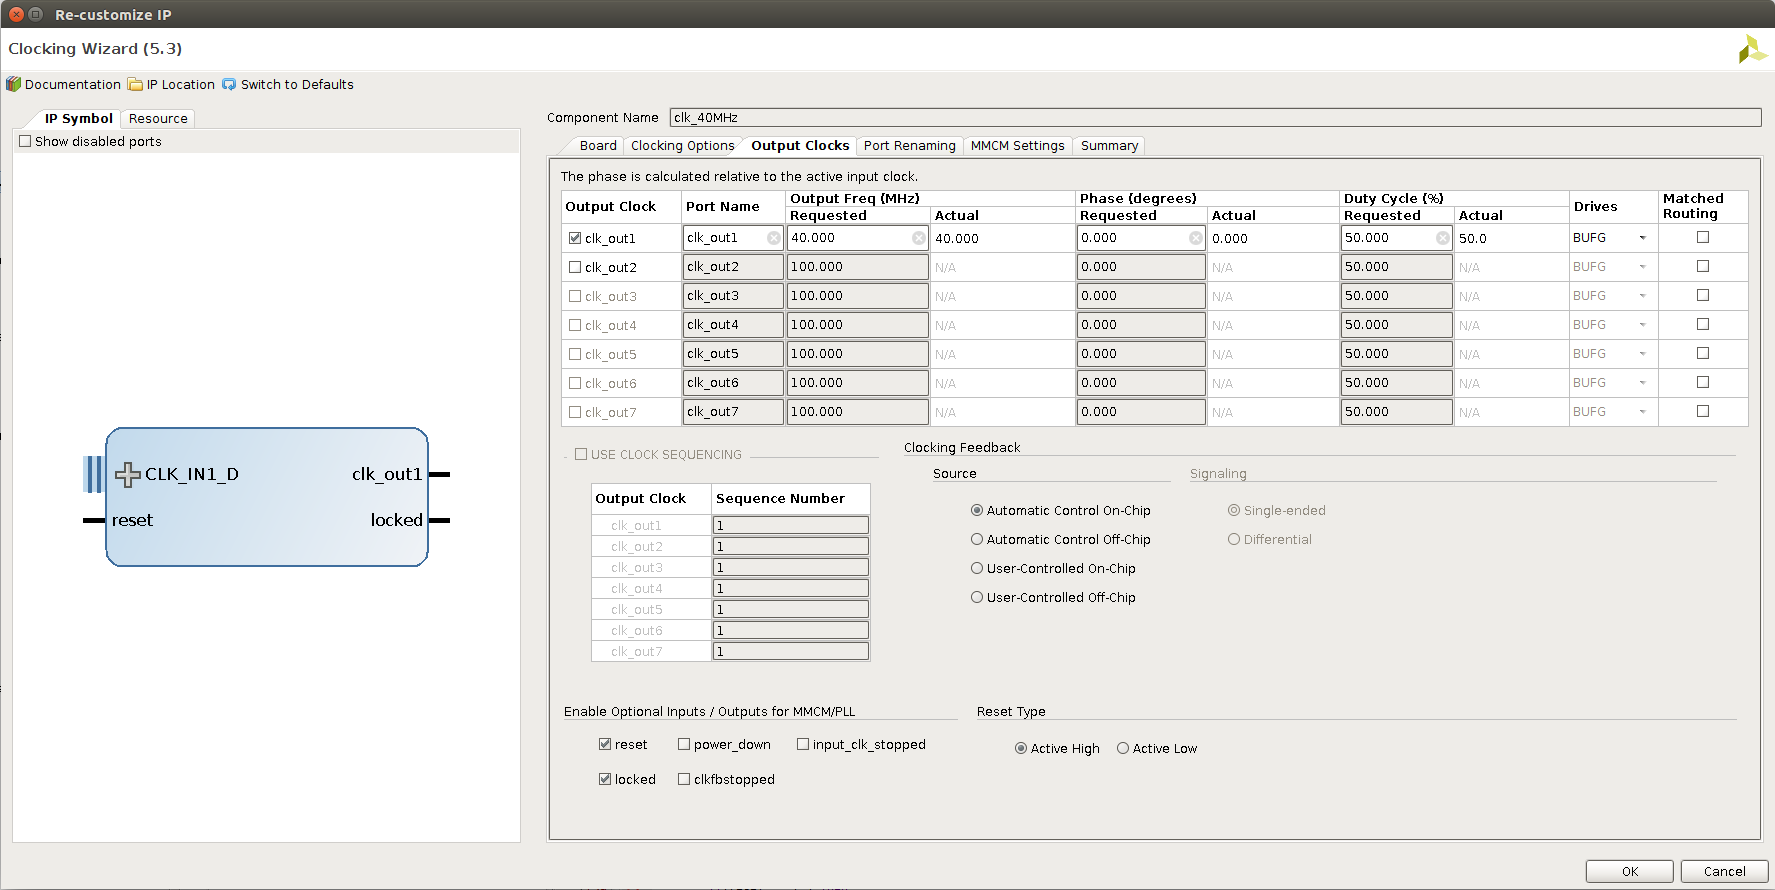
\includegraphics[width=\textwidth]{Core1990/IP_CLK40Conf3.png}	
		\caption{Clocking wizard summary}
		\label{fig:IP_CLK40Conf3}
	\end{figure}
	
	\newpage

\subsection{FIFO IP Cores}
	The Core1990 design contains two FIFO's which are used for the to be transmitted and received data. These two FIFO's have a different purpose but their configurations are nearly identical. This is why they are both described in one section.\\
	
	The TX side FIFO stores all user data transmitted to the interface. Configuring the FIFO starts at the basic tab which allows the user to define the interface type and implementation of the FIFO. Figure \ref{fig:IP_FIFOTXConf1} depicts the first tab. In this case the native interface is used in combination with an independent clocks distributed RAM and two synchronization stages. This way the FIFO can also be used for data crossing clock domains.
	
	\begin{figure}[H]
		\centering
		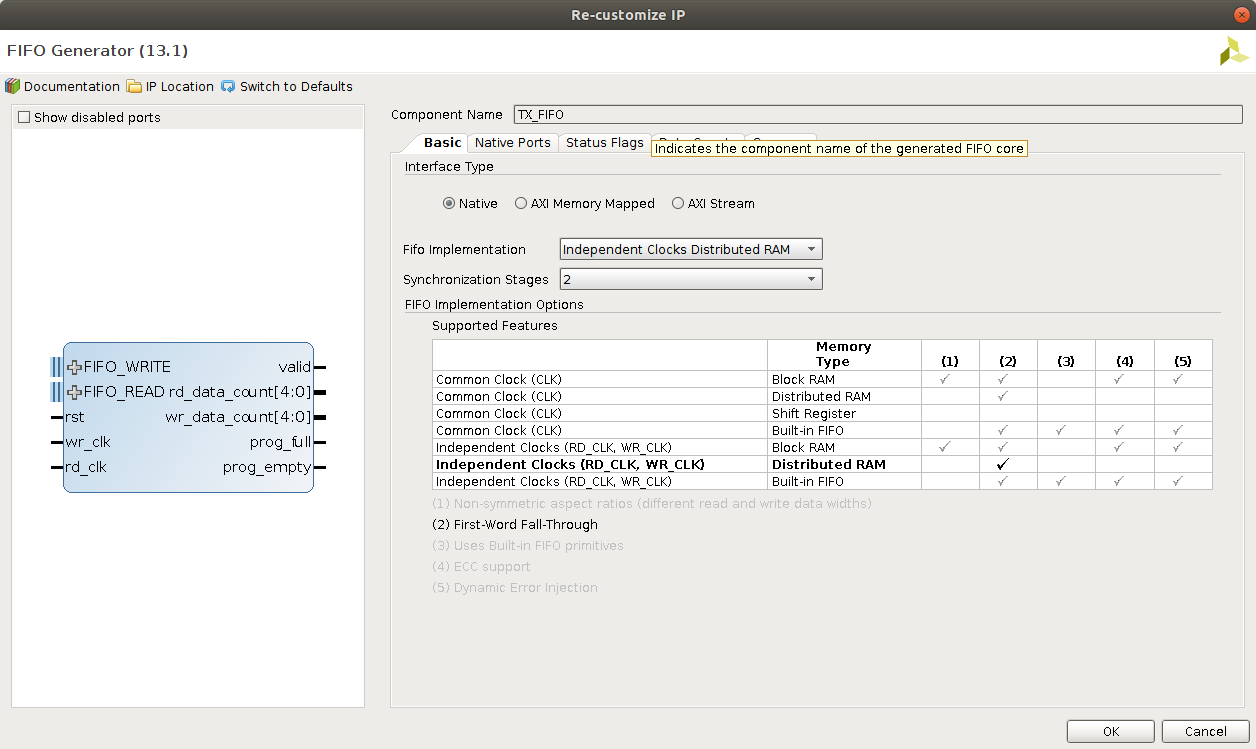
\includegraphics[width=\textwidth]{Core1990/IP_FIFOTXConf1.png}	
		\caption{FIFO generator basic settings}
		\label{fig:IP_FIFOTXConf1}
	\end{figure}
	
	The second configuration tab, as seen in Figure \ref{fig:IP_FIFOTXConf2}, offers more settings on the data width, read mode and initialization. This is meant as a standard FIFO so this option is selected, the only difference with the other mode is interface has to wait one clock cycle after read enable contains a logic high input.\\ 
	
	The FIFO has a data width of 69 bits. This value has been chosen because all essential information now fits in a single packet entering the FIFO. Such packet fits the user data, Start Of Packet, End Of Packet and End Of Packet validbytes. \\
	
	The write depth of the FIFO can be selected according to user preference. In the example 32 packets have been chosen to be sure enough space is available but this could possibly be lowered. Besides this the FIFO contains a reset pin and the output resets to zero. The reset is also synchronized in the core.
	
	\begin{figure}[H]
		\centering
		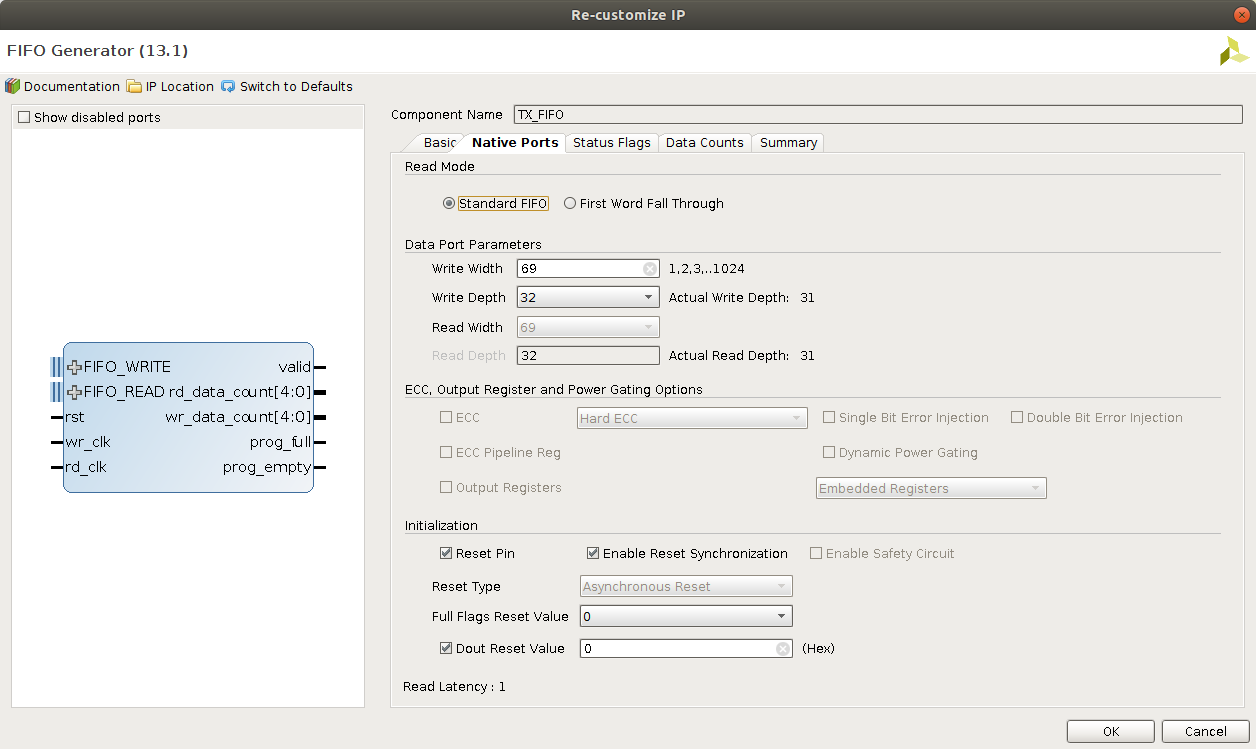
\includegraphics[width=\textwidth]{Core1990/IP_FIFOTXConf2.png}	
		\caption{FIFO generator data port and initialization configuration}
		\label{fig:IP_FIFOTXConf2}
	\end{figure}
	
	In the third tab, depicted in Figure \ref{fig:IP_FIFOTXConf3}, several status flags can be enabled which are very useful. The read port for example uses a valid flag in case the data is really valid. This prevents the interface to transmit duplicated while there is no new data. When valid is a logic low then data will not be read. There are also a few valid programmable flags. In this case Multiple Programmable Full Threshold Constants are used which are useful in combination with flow control.
	
	\begin{figure}[H]
		\centering
		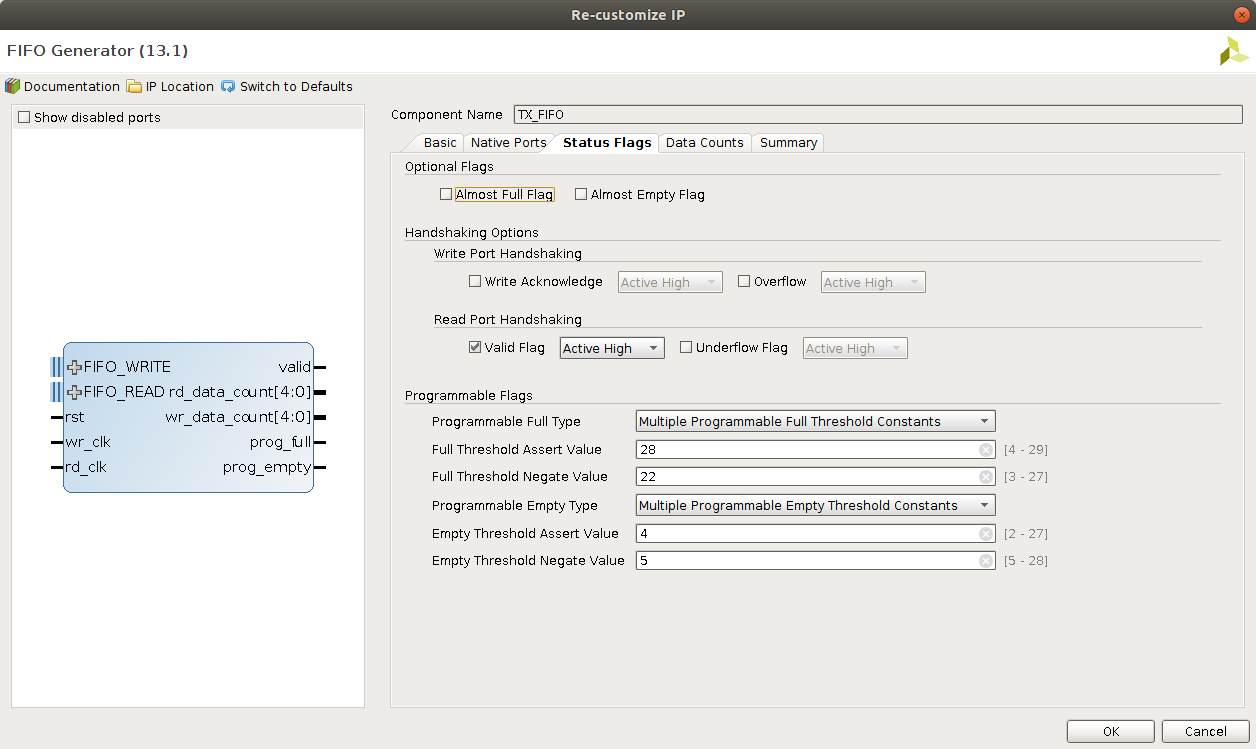
\includegraphics[width=\textwidth]{Core1990/IP_FIFOTXConf3.png}	
		\caption{FIFO generator status flags}
		\label{fig:IP_FIFOTXConf3}
	\end{figure}
	
	The fourth tab contains setting on reading the data count in the FIFO. As usual a summary like the one depicted in Figure \ref{fig:IP_FIFOTXConf4} will always be visible in the last tab. Here you can check whether the necessary settings are configured correctly.
	\begin{figure}[H]
		\centering
		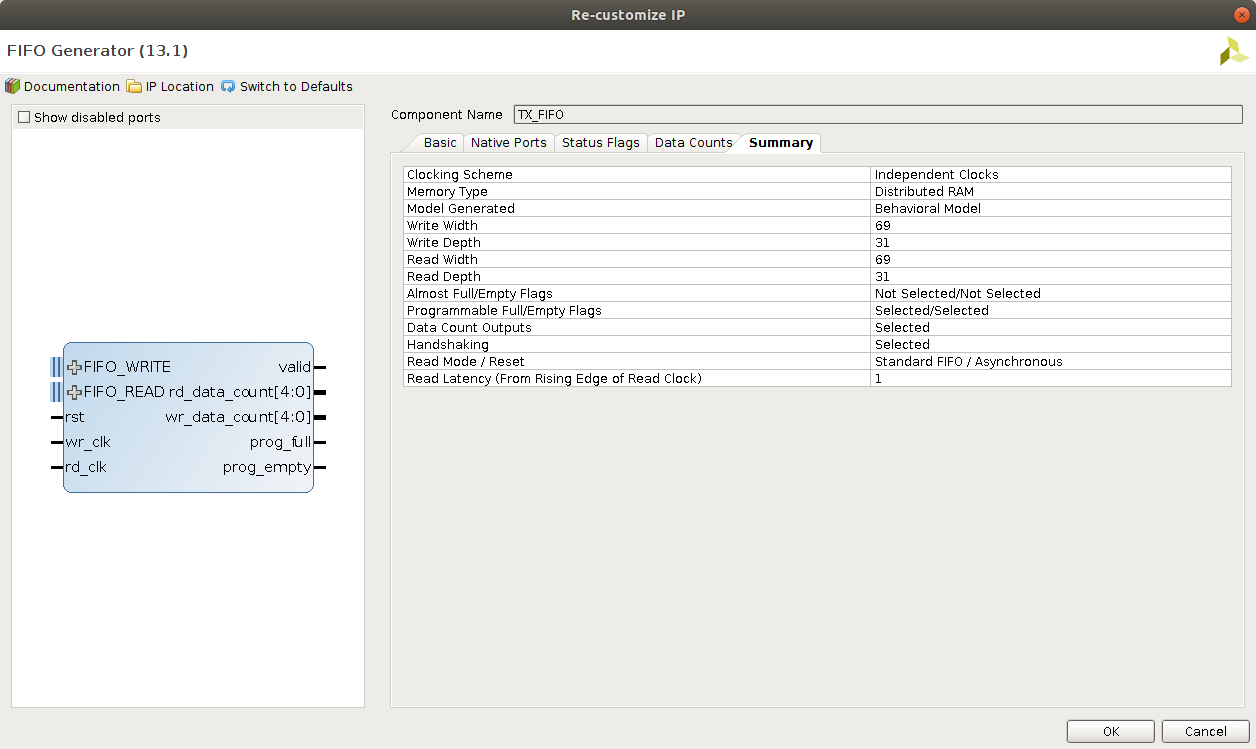
\includegraphics[width=\textwidth]{Core1990/IP_FIFOTXConf4.png}	
		\caption{FIFO generator summary}
		\label{fig:IP_FIFOTXConf4}
	\end{figure}
	
	\newpage
\subsection{Example design}
	\label{Appendix:Core1990_ExampleDesign}
	During the design stage of Core1990 multiple tests have been run to inspect how the link behaves, whether the correct data arrives or how robust the link itself is. These tests have been performed by implementing a data generator connected to the Core1990 inputs. A VIO (Virtual Input/Output) is used to control the length of bursts and an ILA (Integrated Logic Analyzer) is used to sample the input and output data (ChipScope). The input data will be pipelined for alignment between the two. This will make it easier to detect errors and ensure data integrity.
	
	The example design can be generated by running the 'source ./vivado\_import\_virtex7\_exa\\mpledesign.tcl' command from the tcl console.
	
	\begin{forest}
		pic dir tree,
		where level=0{}{% folder icons by default; override using file for file icons
			directory,
		},
		[Core1990
			[constraints]
			[scripts]
			[simulation]
			[sources
				[ip\_cores
					[ILA.xci, file]
					[vio.xci, file] ]
				[tests
					[Core1990\_Test.vhd, file]
					[data\_generator.vhd, file] 
					[pipeline.vhd, file] ]	] ]
	\end{forest}

	\vspace{2mm}
	The additional IP cores and VHDL components are all included in the Core1990\_Test.vhd file. This top level only requires two clocks to run, two differential signals for RX and TX are defined and two output signals indicating locked status and valid compared data are used and connected to an external led. However during testing another clock appeared to be better suited for this purpose (156,25 MHz from the Si570). This requires two additional in- and outputs which are added in the Core1990 file.\\

	The example design realized in Vivado for the VC707 uses 6861 LUT (LookUp Tables), 15599 FF (FlipFlops) and 89 BRAM (Block RAM). Power consumption of the complete design is about 1,3 W.
	\begin{figure}[H]
		\centering
		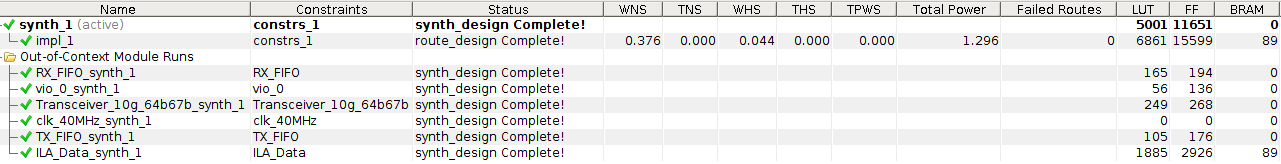
\includegraphics[width=\textwidth]{Core1990/Core1990_ExDesUsage.png}	
		\caption{Resource usage by the example design}
		\label{fig:Core1990_ExDesUsage}
	\end{figure}

	When the example design is opened in Vivado the structure of the project should look similar to what is depicted in Figure \ref{fig:Core1990_VivadoExDes}.
		
	\begin{figure}[H]
		\centering
		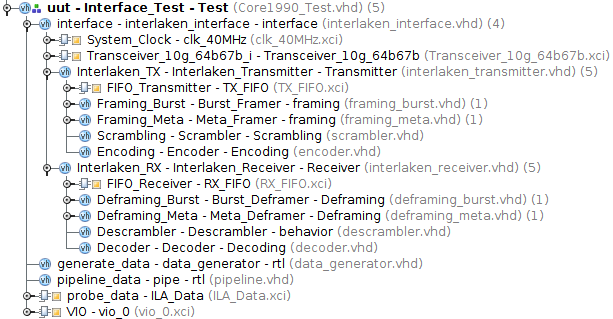
\includegraphics[width=\textwidth]{Core1990/Core1990_VivadoExDes.png}	
		\caption{Structure of the example design in Vivado}
		\label{fig:Core1990_VivadoExDes}
	\end{figure}
	

	\newpage
	
	\subsection{Simulating the core}
	If the link doesn't behave as expected or is malfunctioning, the situation can be analyzed in simulation. This simplifies the process of locating errors.
	Simulation of the core1990 protocol can easily be configured by running the simulation script. This can be done by browsing to the scripts folder again and running the tcl command 'source simulation.tcl'. After this a short explanation of the command this script accepts should appear. For example if the user would like to simulate the decoder, this can be done by giving the command 'simulate decoder' in the tcl console. Simulation of the interface itself van be done by 'simulate interface' and to simulate the example design it is 'simulate core1990'.\\
	
	When running the simulation.tcl script all testbenches will be added to the project. Besides running a specific command to simulate a part it is of course also possible to just start a simulation by selecting the top level in the Vivado GUI in the simulation sources. All added testbench files and the waveform configuration file can be seen in Figure \ref{fig:Core1990_Simulation}.
	
	\begin{figure}[H]
		\centering
		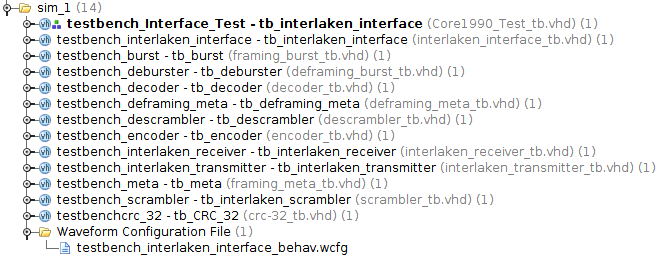
\includegraphics[width=\textwidth]{Core1990/Core1990_Simulation.png}	
		\caption{Structure of the simulation files in Vivado}
		\label{fig:Core1990_Simulation}
	\end{figure}
	